\chapter{File System Recognizer}
\label{cha:fileSystemRecognizer}

%----------
\section{Overview}
This Chapter describes what a file system recognizer is and how it works. The original version is called ExtFsr and was programmed by Matt Wu \href{mailto:mattwu@163.com}{mattwu@163.com} and was only able to recognize ext2 and load the belonging driver. More information about this is available on his website \cite{ext2fsd}.

The functionality was enhanced to differentiate between ext2 and ext3 and then loading the appropriate driver.

%----------
\section{What a file system recognizer is}
A file system recognizer is a standard kernel mode driver like every file system driver. It looks at physical media devices and if it recognizes the media format it loads the appropriate full file system driver. The advantage of such a driver is that it needs less memory than a full file system driver. Some full file system driver might never be required, therefore a small driver like a file system recognizer can save several hundred kilobytes of system memory.

%----------
\section{Start and mount procedure}
Depending on the settings in the registry, the driver will be loaded on system boot process. Otherwise the driver can be loaded by the command \verb~net start extfsr~ manually, given the fact the driver has an entry in the registry.

A mount request will be triggered when windows accesses a not yet mounted partition. When the recognizer receives such a request, it checks the magic number in the super block to decide if it is able to handle the partition. If yes, it checks if journaling is used by the file system.

If ext3 is recognized and a try to load the driver fails, the recognizer tries to load the ext2 driver. That's possible because a ext3 partition is fully accessible through a ext2 driver.

\begin{figure}[H]
\begin{center}
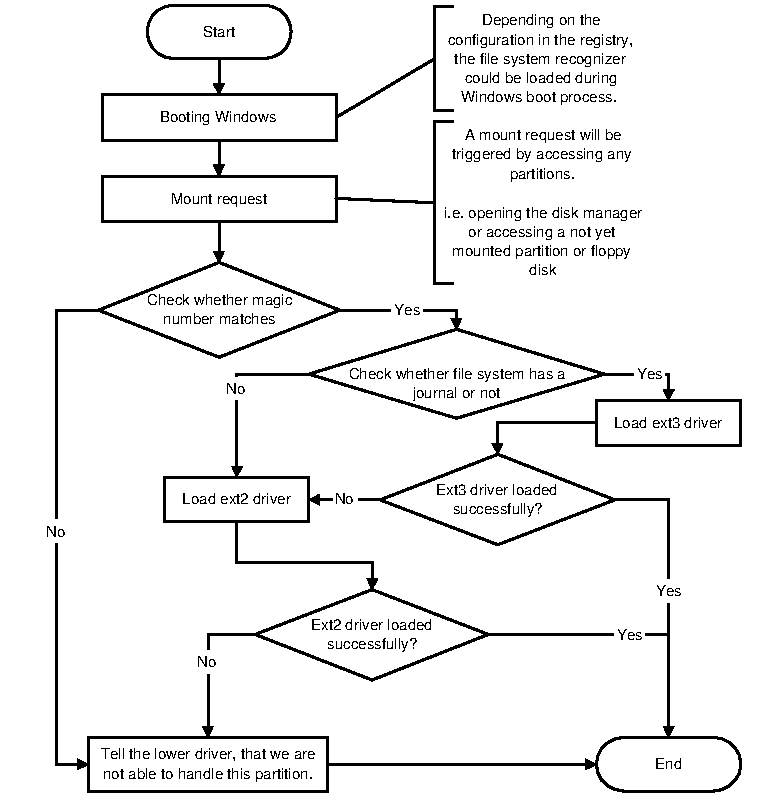
\includegraphics[width=10.9cm]{./files/inc/pic/techRep_FsRec_Overview}
\end{center}
\caption{\label{fig:techRep_FsRec_Overview}Start and mount procedure}
\end{figure}

%----------
\section{How to recognize a ext file system}
First, while initializing the driver, it creates a ``disk file system device'' and registers it as a file system.

\begin{Verbatim}
Status = IoCreateDevice(
  DriverObject,
  sizeof(ExtFsrDeviceExtension),
  &driverName,
  FILE_DEVICE_DISK_FILE_SYSTEM,
  0,
  FALSE,
  &ExtFsrDeviceObject
);

IoRegisterFileSystem(ExtFsrDeviceObject);
\end{Verbatim}

From now on a mount request will reach our file system recognizer when a lower driver calls IoCallDriver with an IRP\_\-MJ\_\-FILE\_\-SYSTEM\_\-CONTROL. To handle such requests, we will have to register the function FileSystemControl as follow:

\begin{Verbatim}
DriverObject->MajorFunction[IRP_MJ_FILE_SYSTEM_CONTROL]=FileSystemControl;
\end{Verbatim}

The Irp Minor Value will be IRP\_\-MN\_\-MOUNT\_\-VOLUME when windows tries to mount a new partition. The FileSystemControl function will read the superblock and compare the magic number. The magic number of ext2 and ext3 is 0xef53 (little-endian) or 0x53ef (big-endian). It can be accessed by the struct of the super block (\verb~ext3_super_block->s_magic~). The following dump shows the place of the magic number in the super block.

\begin{figure}[H]
\begin{center}
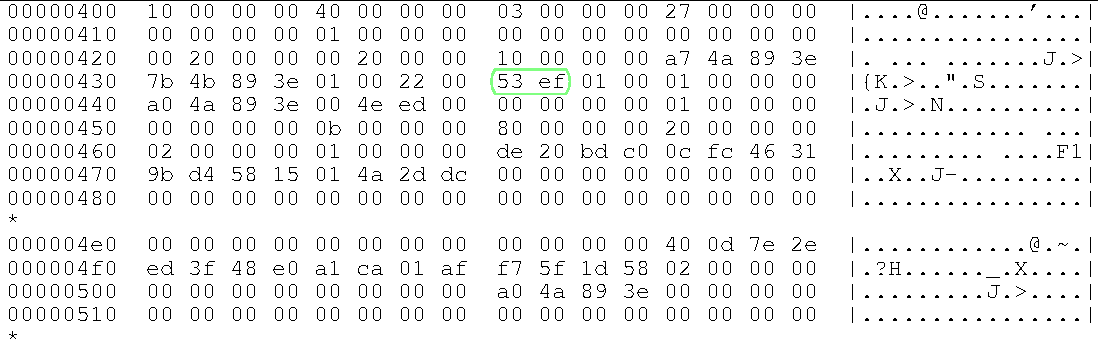
\includegraphics[width=\linewidth]{./files/inc/pic/techRep_FsRec_MagicNumber}
\end{center}
\caption{\label{fig:techRep_FsRec_MagicNumber}Dump of a Super Block with Magic Number}
\end{figure}

\noindent
If the super block, returned by the LoadSuperBlock function, contains the correct ext magic number, the status will be set to STATUS\_\-FS\_\-DRIVER\_\-REQUIRED. Whether the partition is an ext2 or an ext3 partition is decided by checking the journal flag. This flag is set with the third bit of \verb~ext3_super_block->s_feature_compat~

\begin{Verbatim}
// definition of the macro and mask
#define EXT3_FEATURE_COMPAT_HAS_JOURNAL  0x0004
#define EXT3_HAS_COMPAT_FEATURE(sb,mask) \
                               ( sb->s_feature_compat & mask )
                               
// usage of this macro                               
if( EXT3_HAS_COMPAT_FEATURE(ExtSuperBlock, \
                               EXT3_FEATURE_COMPAT_HAS_JOURNAL) )
{
  // some code
}
\end{Verbatim}

The recognized file system version and whether the full file system drivers are loaded or failed is written to the device extension struct of this DeviceObject. The device extension struct is a self declared struct to save device object relevant properties.

If STATUS\_\-FS\_\-DRIVER\_\-REQUIRED is returned to the lower driver, it will call FileSystemControl again but with Irp Minor Value IRP\_\-MN\_\-LOAD\_\-FILE\_\-SYSTEM. Now the recognizer tries to load the full file system driver for ext2 or ext3 depending on the recognized version memorised in the device extension.

\begin{Verbatim}
if (Extension->journaling)
{
  RtlInitUnicodeString(&RegistryPath, EXT3FSD_REGISTRY_PATH);
}
else if (!Extension->journaling)
{
  RtlInitUnicodeString(&RegistryPath, EXT2FSD_REGISTRY_PATH);
}

Status = ZwLoadDriver(&RegistryPath);
\end{Verbatim}

When both driver, ext2 and ext3, have either loaded or failed, the recognizer will first unregister itself as a file system. So it will no longer receive mount requests. Then it deletes the device object and gives the command to unload itself from the system.

\begin{Verbatim}
if(    (Extension->ext2.loaded || Extension->ext2.failed)
    && (Extension->ext3.loaded || Extension->ext3.failed) )
{
  IoUnregisterFileSystem(ExtFsrDeviceObject);
  IoDeleteDevice(ExtFsrDeviceObject);
  RtlInitUnicodeString(&RegistryPath, EXTFSR_REGISTRY_PATH);
  ZwUnloadDriver(&RegistryPath);
}
\end{Verbatim}

%-----
\section{FileSystemControl}
Diagram \ref{fig:techRep_FsRec_FileSystemControl} shows the way to handle a mount request to the recognizer. If the first call to this function with IRP\_\-MN\_\-MOUNT\_\-REQUEST will return STATUS\_\-FS\_\-DRIVER\_\-REQUIRED, we will receive a second request with IRP\_\-MN\_\-LOAD\_\-FILE\_\-SYSTEM. Only on second pass a file system will be loaded if everything went right.
\clearpage

\begin{figure}[H]
\begin{center}
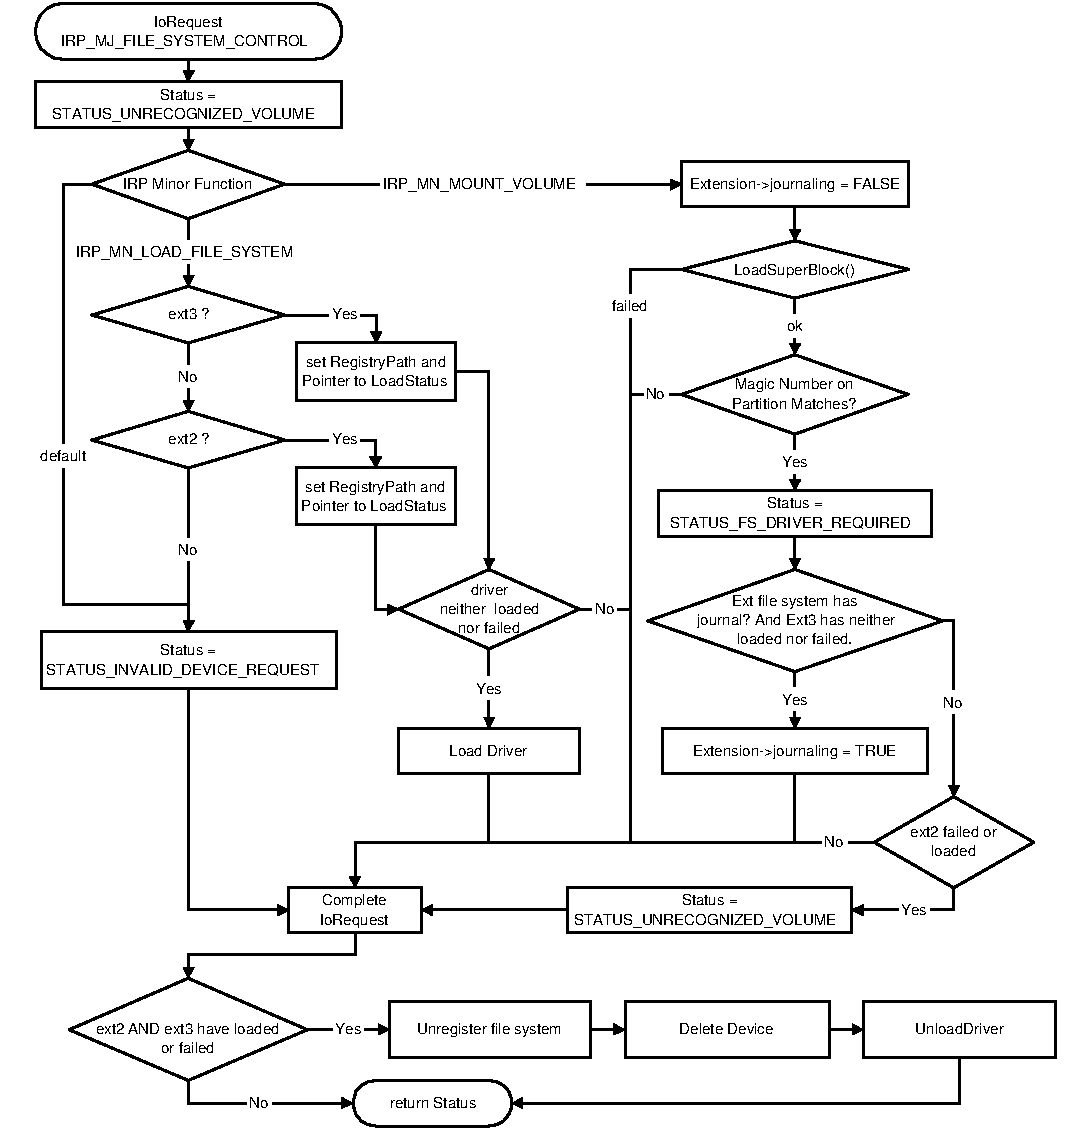
\includegraphics[width=\linewidth]{./files/inc/pic/techRep_FsRec_FileSystemControl}
\caption{\label{fig:techRep_FsRec_FileSystemControl}File System Control Diagram}
\end{center}
\end{figure}


